\recipe{Pancakes, Fluffy}
\label{rec:pancakes_fluffy}
\worktime{30 minutes}
\totaltime{30 minutes}
\makes{Makes enough for one hungry person}
\source{From Ram}

\begin{ingredients}
    \item Flour, \SI{1}{\cup}
    \item Brown sugar, \SI{2}{\tablespoon}
    \item Baking powder, \SI{1.5}{\teaspoon}
    \item Baking soda, \SI{0.5}{\teaspoon}
    \item Salt, \SI{0.25}{\teaspoon}
    \item Eggs, 2 large, yolks separated
    \item Yoghurt, \SI{1}{\cup} Greek
    \item Milk, \SI{0.25}{\cup}
    \item Vanilla extract, \SI{1}{\teaspoon}
\end{ingredients}

\begin{method}
Mix together dry ingredients and wet ingredients separately, reserving the egg whites.

Beat the egg whites to soft peaks. Combine wet and dry ingredients and fold in the beaten egg whites.

Fry.
\end{method}


\begin{figure}[h]
  	\centering
  	
  	\begin{tikzpicture}
  		% Save the image in a box to get its dimensions
  		\sbox0{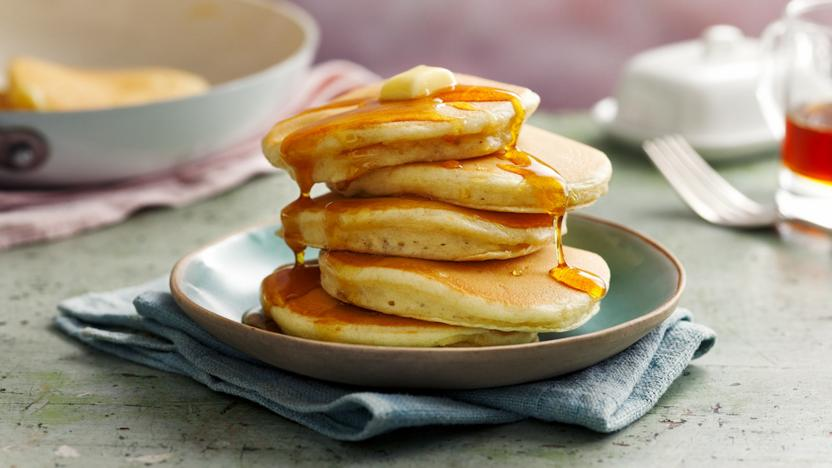
\includegraphics[height=0.45\linewidth]{images/fluffyamericanpancak_74828_16x9.jpg}}%
  
  		% Draw a clipping rectangle with rounded corners
  		\path[clip, rounded corners=0.5cm] (0,0) rectangle (\wd0,\ht0);
  
  		% Place the image inside the clipped area
  		\node[inner sep=0pt, outer sep=0pt, anchor=south west] at (0,0) {\usebox0};
	\end{tikzpicture}

  \caption*{}
\end{figure}